% Opsætter KU Tex dokument
%%%%%%%%%%%%%%%%%%%%%%%%%%%%%%%%%%%%%%%%%%%%%%%%%%%%%%%%%%%%%%%%%%%%%%%%%%%%%%%%
\documentclass{article}                                                        %
\usepackage[a4paper, hmargin={2.8cm, 2.8cm}, vmargin={2.5cm, 2.5cm}]{geometry} %
\usepackage{eso-pic}  % \AddToShipoutPicture                                   %
\usepackage{graphicx} % \includegraphics                                       %
\usepackage{subfig}    
\usepackage{setspace}                                                        %
%%%%%%%%%%%%%%%%%%%%%%%%%%%%%%%%%%%%%%%%%%%%%%%%%%%%%%%%%%%%%%%%%%%%%%%%%%%%%%%%

% Pakker til skrifttyper, tekst osv.
%%%%%%%%%%%%%%%%%%%%%%%%%%%%%%%%%%%%%%%%%%%%%%%%%%%%%%%%%%%%%%%%%%%%%%%%%%%%%%%%
    \usepackage[utf8]{inputenc}  % Implementere Unicode                        %
    \usepackage[T1]{fontenc}     % Unicode skrifttype fx. é skrives som 1 tegn %
    %\usepackage[danish]{babel}   % Dansk Ordbog                                %
    \usepackage{microtype}       % Forbedre linjeombrydningen                  %
    \usepackage{libertine}       % Skrifttype                                  %
%%%%%%%%%%%%%%%%%%%%%%%%%%%%%%%%%%%%%%%%%%%%%%%%%%%%%%%%%%%%%%%%%%%%%%%%%%%%%%%%

% Pakker til matematik og kode.
%%%%%%%%%%%%%%%%%%%%%%%%%%%%%%%%%%%%%%%%%%%%%%%%%%%%%%%%%%%%%%%%%%%%%%%%%%%%%%%%
    \usepackage{mathtools}       % Udvidelse til amsmath pakken                %
    \usepackage{amsthm}          % Pakke til bevisførelse                      %
    \usepackage{amssymb}         % Extra matematiske symboler                  %				
	\usepackage{mychemistry}												   %
	\usepackage[version=3]{mhchem}											   %
	\usepackage{wrapfig}													   %
	\usepackage{siunitx}	
	\usepackage{anyfontsize}
	\usepackage{url}
	\usepackage{ragged2e}
	\usepackage{algorithm2e}
	\usepackage[final]{pdfpages}
	\usepackage{listings}
	\usepackage{tikz}
	\usepackage{multirow}
	\usepackage{makecell}
	\usepackage{fourier} 
	\usepackage{array}
	\usepackage{todonotes}
	\usepackage{pdflscape}
	\usetikzlibrary{arrows,shapes}
	\usepackage{titlesec}
	\usepackage{hyperref}
	\usepackage{url}
	\usepackage[nottoc,numbib]{tocbibind}
	
	\urlstyle{same}
	\tikzstyle{vertex}=[circle,fill=white!25,minimum size=20pt,inner sep=0pt]
	\tikzstyle{edge} = [draw,thick,-]

	\definecolor{light-gray}{gray}{0.85}
	\definecolor{dkgreen}{RGB}{0.0,128.0,43.0}
	\lstdefinelanguage{FSharp}%
{morekeywords={new, match, with, rec, open, module, namespace, type, of, member, % 
and, for, while, true, false, in, do, begin, fun, function, return, yield, try, %end
mutable, if, then, else, cloud, async, static, use, abstract, interface, inherit, finally, int },
  otherkeywords={ let!, return!, do!, yield!, use!, var, from, select, where, order, by },
  keywordstyle=\color{bluekeywords},
  sensitive=true,
  basicstyle=\ttfamily,
	breaklines=true,
  xleftmargin=\parindent,
  aboveskip=\bigskipamount,
	tabsize=4,
  morecomment=[l][\color{dkgreen}]{///},
  morecomment=[l][\color{dkgreen}]{//},
  morecomment=[l][\color{dkgreen}]{(*},
  morecomment=[s][\color{dkgreen}]{},
  morestring=[b]",
  showstringspaces=false,
  literate={`}{\`}1,
  stringstyle=\color{redstrings},
}
	
	\lstset{frame=tb,
  	language=FSharp,			%CHANGE LANGUAGE
  	aboveskip=3mm,
  	belowskip=3mm,
  	showstringspaces=false,
  	columns=flexible,
  	basicstyle={\small\ttfamily},
  	numbers=none,
  	numberstyle=\tiny\color{gray},
  	keywordstyle=\color{blue},
  	commentstyle=\color{dkgreen},
  	stringstyle=\color{red},
  	breaklines=true,
  	breakatwhitespace=true,
  	tabsize=3,
  	backgroundcolor=\color{light-gray},
	}
												   %
%%%%%%%%%%%%%%%%%%%%%%%%%%%%%%%%%%%%%%%%%%%%%%%%%%%%%%%%%%%%%%%%%%%%%%%%%%%%%%%%

% Pakker til layout.
%%%%%%%%%%%%%%%%%%%%%%%%%%%%%%%%%%%%%%%%%%%%%%%%%%%%%%%%%%%%%%%%%%%%%%%%%%%%%%%%
    \usepackage{fancyhdr}            % Gør det muligt at bruge sidehoveder     %
    \usepackage{graphicx}            % Mulighed for bl.a. \includegraphics     %
    \usepackage{colortbl}            % Hvis man vil farvelægge sine tabeller   %
    \usepackage{array}               % Gør miljøerne array og tabular bedre    %
    \usepackage{parskip}             % Første paragraf i afsnit indrykkes ikke %
    \usepackage{titlesec}            % Tilpassing af afstand mellem sektioner  %
    \usepackage[lastpage,user]{zref} % Side x af y                             %
%%%%%%%%%%%%%%%%%%%%%%%%%%%%%%%%%%%%%%%%%%%%%%%%%%%%%%%%%%%%%%%%%%%%%%%%%%%%%%%%


% Implementerer en række makroer og de pakker der er importeret
%%%%%%%%%%%%%%%%%%%%%%%%%%%%%%%%%%%%%%%%%%%%%%%%%%%%%%%%%%%%%%%%%%%%%%%%%%%%%%%%
    \pagestyle{fancy}                        % Implementerer sidehoved         %
    \lhead{University of Copenhagen}                % Venstre sidehoved               %
    \rhead{Casper Bresdahl, Karl Levinsen}                             % Højre sidehoved      %
    \cfoot{\thepage\ of \zpageref{LastPage}} % Side x af y                     %
    \newtheorem*{prp}{Propostion}            % Skaber nyt theorem  
    \renewcommand{\baselinestretch}{1.5}       %
%%%%%%%%%%%%%%%%%%%%%%%%%%%%%%%%%%%%%%%%%%%%%%%%%%%%%%%%%%%%%%%%%%%%%%%%%%%%%%%%

% Mindsker afstanden mellem sektioner
%%%%%%%%%%%%%%%%%%%%%%%%%%%%%%%%%%%%%%%%%%%%%%%%%%%%%%%%%%%%%%%%%%%%%%%%%%%%%%%%%%
\titlespacing\section{0pt}{12pt plus 4pt minus 2pt}{0pt plus 1pt minus 3pt}      %
\titlespacing\subsection{0pt}{12pt plus 4pt minus 2pt}{0pt plus 1pt minus 3pt}   %
\titlespacing\subsubsection{0pt}{12pt plus 4pt minus 2pt}{0pt plus 1pt minus 3pt}%
%%%%%%%%%%%%%%%%%%%%%%%%%%%%%%%%%%%%%%%%%%%%%%%%%%%%%%%%%%%%%%%%%%%%%%%%%%%%%%%%%%

%Ændrer størelsen på sections
%%%%%%%%%%%%%%%%%%%%%%%%%%%%%%%%%%%%%%%%%%%%%%%%%%%%%%%%%%%%%%%%%%%%%%%%%%%%%%%%%%
\titleformat{\section}
{\normalfont\fontsize{14}{16}\bfseries}{\thesection}{1em}{}
\titleformat{\subsection}
{\normalfont\fontsize{12}{14}\bfseries}{\thesubsection}{1em}{}
\titleformat{\subsubsection}
{\normalfont\fontsize{11}{13}\bfseries}{\thesubsubsection}{1em}{}
%%%%%%%%%%%%%%%%%%%%%%%%%%%%%%%%%%%%%%%%%%%%%%%%%%%%%%%%%%%%%%%%%%%%%%%%%%%%%%%%%%

%%%%%%%%%%%%
% Document %
%%%%%%%%%%%%

\begin{document}

\begin{titlepage}

\newcommand{\HRule}{\rule{\linewidth}{0.5mm}} % Defines a new command for the horizontal lines, change thickness here

\begin{center}
 % Center everything on the page
 
%----------------------------------------------------------------------------------------
%	HEADING SECTIONS
%----------------------------------------------------------------------------------------

\textsc{\LARGE University of Copenhagen}\\[1.5cm] % Name of your university/college
\textsc{\Large Computer Science}\\[0.5cm] % Major heading such as course name
\textsc{\large Bachelor Thesis}\\[0.5cm] % Minor heading such as course title

%----------------------------------------------------------------------------------------
%	TITLE SECTION
%----------------------------------------------------------------------------------------

\HRule \\[0.4cm]
{ \huge \bfseries Synthesis of Actor Code and tests =====TBD======}\\[0.4cm] % Title of your document
\HRule \\[1.5cm]
 
%----------------------------------------------------------------------------------------
%	AUTHOR SECTION
%----------------------------------------------------------------------------------------

\begin{minipage}{0.4\textwidth}
\begin{flushleft} \large
\emph{Authors:}\\ 
% Your name
Casper \textsc{Bresdahl} \\
Karl \textsc{Levinsen}
\end{flushleft}
\end{minipage}
~
\begin{minipage}{0.4\textwidth}
\begin{flushright} \large
\emph{Supervisor:} \\
Boris \textsc{Düdder}\\
\hfill
\end{flushright}
\end{minipage}\\[2cm]

% If you don't want a supervisor, uncomment the two lines below and remove the section above
%\Large \emph{Forfattere:}\\
%Axel \textsc{Christof}\\% Your name
%Casper \textsc{Bresdahl}\\
%Emilie \textsc{Bentsen}\\[1cm] 

%----------------------------------------------------------------------------------------
%	DATE SECTION
%----------------------------------------------------------------------------------------

{\large \today}\\[2cm] % Date, change the \today to a set date if you want to be precise

%----------------------------------------------------------------------------------------
%	LOGO SECTION
%----------------------------------------------------------------------------------------


\includegraphics{logo.png}\\[1cm] % Include a department/university logo - this will require the graphicx package
 
%----------------------------------------------------------------------------------------

\vfill % Fill the rest of the page with whitespace

%Disse linjer skaber forside, evt indholdsfortegnelse, og sætter sidetal
%%%%%%%%%%%%%%%%%%%%%%%%%%%%%%%%%%%%%%%%%%%%%%%%%%%%%%%%%%%%%%%%%%%%%%%%%%%%%%%%
									                                           %
    \thispagestyle{empty}   % Fjerner sidetal forside                          %
        % Slå disse til hvis der ønskes indholdsfortegnelse                    %
        %%%%%%%%%%%%%%%%%%%%%%%%%%%%%%%%%%%%%%%%%%%%%%%%%%%%%%%%%%%%%%%%%%%%%%%% 
            \newpage                % Side til indholdsfortegnelse            %
            \thispagestyle{empty}   % Fjerner sidetal fra indholdsfortegnelse %
            \tableofcontents        % Skaber indholdsfortegnelse              %
    \end{center}
    %\section*{Forord}
    	
		
        %%%%%%%%%%%%%%%%%%%%%%%%%%%%%%%%%%%%%%%%%%%%%%%%%%%%%%%%%%%%%%%%%%%%%%%%
    \newpage                % Første rigtige side
    \setcounter{page}{1}    % Sætter rigtigt sidetal på første side
%%%%%%%%%%%%%%%%%%%%%%%%%%%%%%%%%%%%%%%%%%%%%%%%%%%%%%%%%%%%%%%%%%%%%%%%%%%%%

\end{titlepage}
{\fontsize{10}{14}\selectfont

\section{Introduction} \label{intro}
In this thesis we have extended upon a sandbox like demo project from Microsoft \cite{AdventureGame} which resembles an adventure game and is written in a distributed fashion with Orleans. We have then decomposed it into a code repository with the  purpose of using the Combinatory Logic Synthesizer, a type based tool to automatically compose larger systems from a repository of code components, to create different variations of the game based on definitions written in a metalanguage. Our goal has been to synthesize code with timers, synthesizing code where we dispose timers, synthesizing code where we create other actors and to be able to define a list of parameters in our metalanguage and then synthesize code where only the defined parameters are present in the game variation. Our goal has also been to test our application, both as the initial program as well as the combinated variations of the game. This means synthesizing tests in the same way as our code, such that a given variation has tests alongside the program specific to that variation. 
\todo{Extend introduction to introduce testing?}\\
We will begin by looking at the theory behind the actor model and Orleans, then we will move to the theory of the Combinatory Logic Synthesizer and how it works. After that we will look into more detail about the extensions we have made to the Microsoft project. We will then look into the design decisions about decomposing the code, the issues we faced and what improvements we could have made. We will also look into what makes a good component and ask ourselves if we have achieved good decomposition. 
Then we will look into the relevant theory of testing software, followed by a deeper dive into our testing, meaning the tests themselves alongside the tests as combinators in the CLS. We will be discussing our implementation and looking at some of the obstacles we faced during our process of creating tests\todo{Change for a more comprehensive description}. We will then comment on our results and lastly make our conclusions.
\begin{itemize}
	\item Abstract
	\item Introduction
	\item Actor model - 4
	\item CLS - 4
	\item Our product - 4
	\item Discussion of implementation - 12
	\item Testing theory - 4
	\item Discussion of testing - 12
	\item Results - 4
	\item Conclusion
\end{itemize}
\section{Actor model}
The actor model is a programming model utilising concurrent computation for developing parallel, distributed and mobile systems. An actor can do three things: it can send messages to other actors, it can update its local state or it can create more actors. All actors work concurrently and asynchronously together by sending and receiving messages. When an actor receives a message it performs some specified task based on its local state and the content of the received message. This task can be to perform some computation, and the result can then be passed along to another actor in a new message \cite{ActorModelPaper}.\\
All actors have a globally unique name which is used to determine to which actor a message is sent. Name of actors may be communicated in messages such that an actor knows who to send the next message to, or such that an actor knows who just sent it a message. An actor's state is local and can not be shared with other actors, and thus, to change the behaviour of an actor, another actor must send a message specifying it to change state. The path a message takes and what network delays a message may encounter is not specified and thus messages may arrive out of order \cite{ActorModelPaper}.\\
\begin{figure}[H]
	\centering
	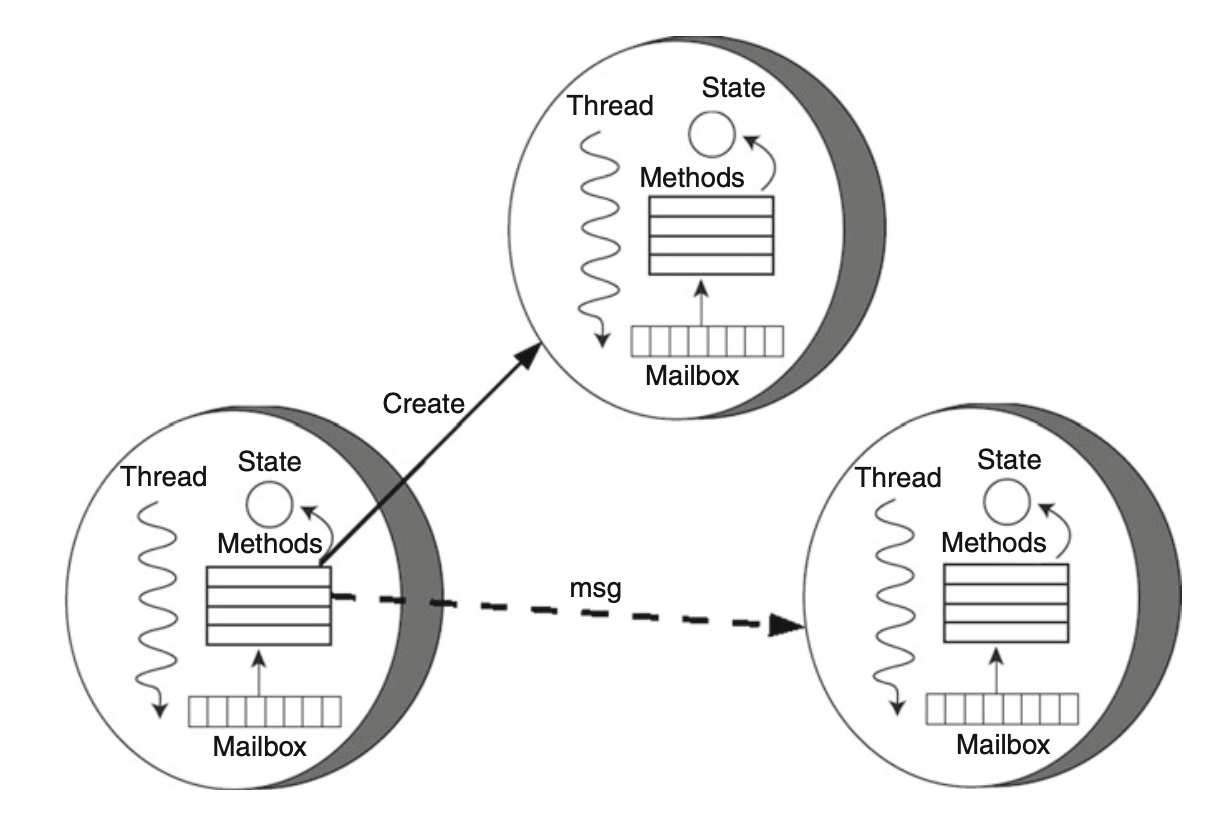
\includegraphics[width=0.85\linewidth]{Materials/ActorModel/AMDemonstrated}
	\caption{An actor consists of methods, a mailbox for queued messages and a local state. Actors can send messages, change state based on a received message and create other actors. Figures is from \cite{ActorModelPaper}.}
	\label{AMDemonstrated}
\end{figure}
As seen in \autoref{AMDemonstrated} an actor can be illustrated as an entity with a mailbox, a set of methods and a local state. The mailbox is often implemented as a queue \cite{ActorModelPaper}, and is used to store messages which arrive while the actor is already handling another message. The methods may make the actor change its state, make the actor create a new actor or send a message to another actor.\\
As already hinted at above, the core semantic properties of an actor are \textit{encapsulation} of the local state, the ability to \textit{atomically} execute methods, \textit{fairness} in scheduling actors and \textit{location transparency} to enable distributed execution and mobility \cite{ActorModelPaper}, and all of these we will look into next.
 
\subsubsection{Encapsulation and Atomicity}
Encapsulation means each actor has its own state, and thus all changes to the state of an actor has to come in a message sent from another actor. The notion of encapsulation is also one of the corner stones of object oriented programming where each object also has its own state. This can be very useful to enforce an object oriented decomposition in code, and may make actors look a lot like objects \cite{ActorModelPaper}.\\
Encapsulation has also lead to the notion of atomicity. In a sequential program one object may call a method in another object. This method will then run to the end before another object can call the method again. The called object may or may not have changed state during the method call, but we can only reason about this because the method call can not be interrupted by another method call. Because all method calls are run uninterrupted, we can reason about the object's behaviour given we know its state prior to the method call \cite{ActorModelPaper}.\\
In a concurrent setting an object may call a method in another object, but right after a third object does the same. If the first method call would be interrupted to accommodate the second, the object's state might already be altered, and we can no longer reason about the behaviour the object exhibits after a call to its method. This would lead to inconsistencies in the system as these concurrent calls can happen at any time. To guarantee we can reason about object behaviour in actors we therefore must guarantee that received messaged are handled atomically, meaning that the processing of a message happens in one step, and is not interrupted by new messages. This ensures that the encapsulated state is consistent throughout the execution of a program \cite{ActorModelPaper}.

\subsubsection{Fairness}
The notion of fairness states that all actors are scheduled time to run, and that they will make progress given they have computations to do. It also states that all messages are guaranteed to reach their destination unless that actor has been permanently disabled. The notion of fairness allows us to reason about the liveness properties of actor programs \cite{ActorModelPaper}. Here we note that an actor program is started by an external message sent to an actor, and that an actor program terminates when all actors are idle and no external message can be passed to any actors. An actor is considered idle if it has no pending messages in its mailbox.

\subsubsection{Location transparency}
Location transparency provides an abstraction for the programmers who need to make actors communicate. In the actor model the location of actors does not determine its name. Two actors might run on the same computer in the same core, or they might run on two different machines in two different countries. Location transparent naming enables the programmers no to worry about the actors physical location. \cite{ActorModelPaper}.\\
Mobility is defined as the ability for a computation to migrate to another node \cite{ActorModelPaper}. This is important for load-balancing, fault-tolerance, and reconfiguration, and is useful in achieving scalable performance \cite{ActorModelPaper} as an actor lifting a lot of heavy work along other actors doing the same on the same machine can seamlessly be moved to another machine in an attempt to alleviate the workload on that machine.

\subsubsection{Synchronization}
\begin{figure}[H]
	\centering
	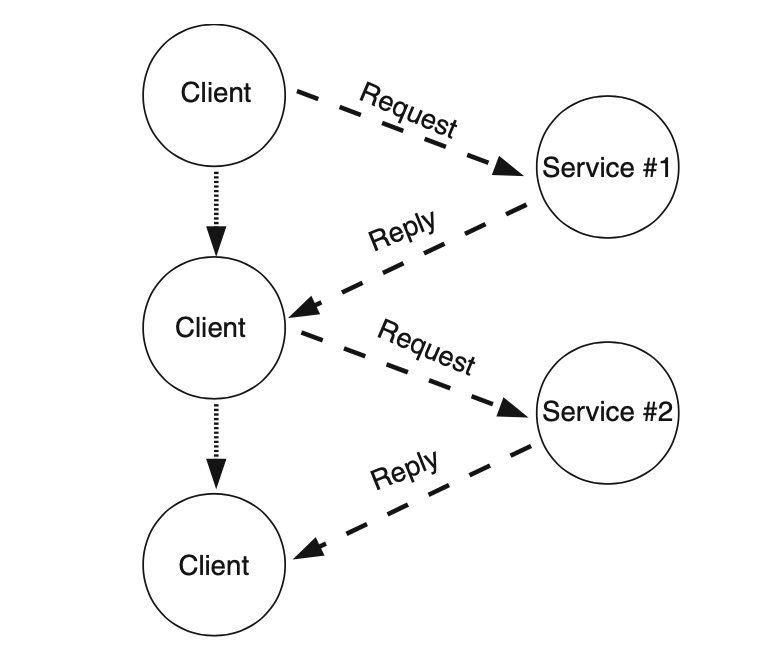
\includegraphics[width=0.6\linewidth]{Materials/ActorModel/AMCommunication}
	\caption{An illustration of how RPC like communication works. Figures is from \cite{ActorModelPaper}.}
	\label{AMCommunication}
\end{figure}
One way to achieve synchronization of actors is through Remote Procedure Call like message passing (RPC), which is a common communication pattern in actor systems \cite{ActorModelPaper}. In a situation where an actor wants to make sure another actor has received its message before it communicates it to others or where the order of messages matter RPC like messaging is a big help. In RPC like communication the sender of a message waits for a reply before it continues to process other messages. An actor might want to wait for a reply if it needs the information in the reply to continue its computation. This can be seen in \autoref{AMCommunication} where the client sends a message to a service and waits for the reply before sending another message to another service \cite{ActorModelPaper}.\\

\subsection{Orleans}
Orleans is a framework for C\# developed by Microsoft. The framework simplifies several aspects of the actor model to make it a lot easier for programmers to write actor based code. Some of the simplifications Orleans helps with are lifecycle management of actors in the application code, to deal with distributed race conditions, to handle failures and recovery of actors after server crashes, and to make an abstraction for actor placement.\\
An important abstraction the developers of Orleans have made is the notion of virtual actors. In Orleans we work with virtual actors which are based on the actors described previously, but they implement some important differences which abstract away some of the more cumbersome implementations of actors. The first of these is perpetual existence which states that virtual actors are logical entities which always exists. A virtual actor can not explicitly be created or destroyed. Its existence is unaffected by the server which runs it, and thus also unaffected by the server crashing. Given that a virtual actor always exists, it is also always addressable \cite{OrleansPaper}.\\
Another great help Orleans implement is automatic instantiation. The Orleans' runtime automatically creates instantiations of actors called activations. An actor can only be instantiated if it has a request pending. When a request is sent to an actor the Orleans runtime automatically instantiates an activation on a server. If the server should later crash, the Orleans runtime automatically re-instantiates the actor when the next request to it arrives. This means that the programmer does not have to program actor lifecycles themselves, but can rely on Orleans to automatically figuring out where and when to instantiate an actor. Likewise, the Orleans runtime also automatically disposes unused actors if they have been idle for a long time \cite{OrleansPaper}.\\
Orleans also takes care of the location transparency abstraction. An application running inside an actor, or communicating with an actor does not know its physical location, and neither does it need to, as long as it knows the actors name it can send it a message. Orleans allow programmers to name actors much like one would name an object in an ordinary object-oriented program.\\
Orleans allows for timers which, as the name suggests, specify code that will be run later. A timer is automatically disposed if an actor is recycled by runtime, but can otherwise be specified to fire in even intervals. Because timers 'run in the background' it is important that the programmer makes sure they are disposed when no longer needed.\\
Orleans allows actors to synchronize through RPC-like message passing as discussed in subsection '\nameref{Synchronization}'. This is done by awaiting a response from another actor. Due to atomicity the actor can not progress its method while awaiting a response. Therefore other actors or other tasks are run in the mean time while the actor waits. When the response arrives the actor will then continue the method from where it left off.
\begin{thebibliography}{9}
\bibitem{ActorModelPaper}
Karmani, Rajesh K. Agha, Gul. Padua, David (ed.). 2011. 'Actors', part of 'Encyclopedia of Parallel Computing'. Springer Science+Business Media. Downloaded: November 26, 2019.

\bibitem{TestingCodeComplete}
McConnell, Steve. 2004. 'Code Complete'. Microsoft Press 2. ed. Chap. 22.

\bibitem{TestingAdaptiveCode}
Hall, Gary. 2014. 'Adaptive Code via C\#'. Microsoft Press 1. ed. Chap. 4.
\bibitem{OrleansPaper}
Bernstein, Philip A. Bykov, Sergey. Geller, Alan. et. al. 2014. 'Orleans: Distributed Virtual Actors for Programmability and Scalability'. Microsoft Research. Available at: \url{www.microsoft.com}. Downloaded: December 8, 2019.

%%%%%%%%%%%%%%%%%%%%%%%%%%%%%%%%%%%%%% SHOULD BE DELETED %%%%%%%%%%%%%%%%%%%%%%%%%%%%%%%%%%%%%%%%%%%%%%
\bibitem{book}
Marchewka, Jack T. 2015. 'Information Technology Project Management - Providing Measurable Organizational Value'. Wiley 5. ed.

\bibitem{rigsrevision}
Rigsrevisionen. 13. september 2019. 'Beretning om udvikling af det nye inddrivelsessystem og tilslutning af fordringshavere'. \url{www.rigsrevisionen.dk}. Hentet: 28. oktober 2019.

\bibitem{ugeopgave2}
Mogensen, Sten. 12. september 2019. 'Ugeopgave 2'. \url{absalon.ku.dk}. Hentet: 28. oktober 2019.

\bibitem{ugeopgave3}
Mogensen, Sten. 19. september 2019. 'Ugeopgave 3'. \url{absalon.ku.dk}. Hentet: 29. oktober 2019.

\bibitem{waterfallVsAgile}
Glowtouch.com. 'Waterfall vs. Agile: The Good, The Bad and The Misunderstood'. \url{https://www.glowtouch.com/waterfall-vs-agile-good-bad-misunderstood/}. Hentet: 29. oktober 2019.

\bibitem{scrumMaster}
Andersen, Tania. 4. januar 2018. 'Agile metoder er i dag den herskende måde at udvikle software på. Men Scrum og andre agile teknikker er ingen garanti for succes'. \url{www.version2.dk}. Hentet: 29. oktober 2019.
%%%%%%%%%%%%%%%%%%%%%%%%%%%%%%%%%%%%%% SHOULD BE DELETED %%%%%%%%%%%%%%%%%%%%%%%%%%%%%%%%%%%%%%%%%%%%%%
\end{thebibliography}

\end{document}